\documentclass[12pt, openany]{report}
\usepackage[utf8]{inputenc}
\usepackage[T1]{fontenc}
\usepackage[a4paper,left=2cm,right=2cm,top=2cm,bottom=2cm]{geometry}
\usepackage[french]{babel}
\usepackage{libertine}
\usepackage[pdftex]{graphicx}
\usepackage{lipsum}

%\setlength{\parindent}{0cm}
\setlength{\parskip}{1ex plus 0.5ex minus 0.2ex}
\newcommand{\hsp}{\hspace{20pt}}
\newcommand{\HRule}{\rule{\linewidth}{0.5mm}}

\begin{document}

\begin{titlepage}
  \begin{rmfamily}
  \begin{center}

    % Upper part of the page. The '~' is needed because \\
    % only works if a paragraph has started.
    ~\\[2cm]

    \textsc{\LARGE Universit\'e Polytechnique Hauts-de-France}~\\[0.5cm]
    \textsc{\LARGE Institut National des Sciences Appliqu\'ees}\\[2cm]

    \textsc{\Large Rapport de projet}\\[2cm]

    % Title
    %\HRule \\[0.4cm]
    { \Huge \bfseries Moteur de jeu pour un jeu de plateforme 2D\\[2cm] }

    %\HRule \\[2cm]
    
\includegraphics[scale=0.8]{uphf.png}
    \\
    
\includegraphics[scale=1]{insa.JPG}
    \\[1cm]

    % Author and supervisor
%    \begin{minipage}{0.4\textwidth}
%      \begin{flushleft} \large
%        Ethan \textsc{MARLOT}\\
%        Promo 2015\\
%      \end{flushleft}
%    \end{minipage}
%    \begin{minipage}{0.4\textwidth}
%      \begin{flushright} \large
%        \emph{Tuteur :} M. Le \textsc{Tuteur}\\
%        \emph{Chef d'équipe : } M. Chef \textsc{D’Équipe}
%      \end{flushright}
%    \end{minipage}

    \vfill

    % Bottom of the page
    {\large Ethan \textsc{MARLOT} - 8 Avril 2022}

  \end{center}
  \end{rmfamily}
\end{titlepage}

\tableofcontents

\chapter{Introduction}
Dans le cadre de ce projet tuteur\'e de cette ann\'ee 2022, j'ai choisi de d\'evelopper un jeu de type "Plateformer-Shooter", similaire aux jeux d'acrade \textit{Metal Slug}. Afin de r\'ealiser ce projet, j'ai d\'ecid\'e de ne pas utiliser un moteur de jeu existant mais d'en cr\'eer une impl\'ementation simple.
\\[0.5cm]
\indent En l'\'etat, voici l'apparence du jeu :\\[0.2cm]
\begin{figure}[!h]
\centering
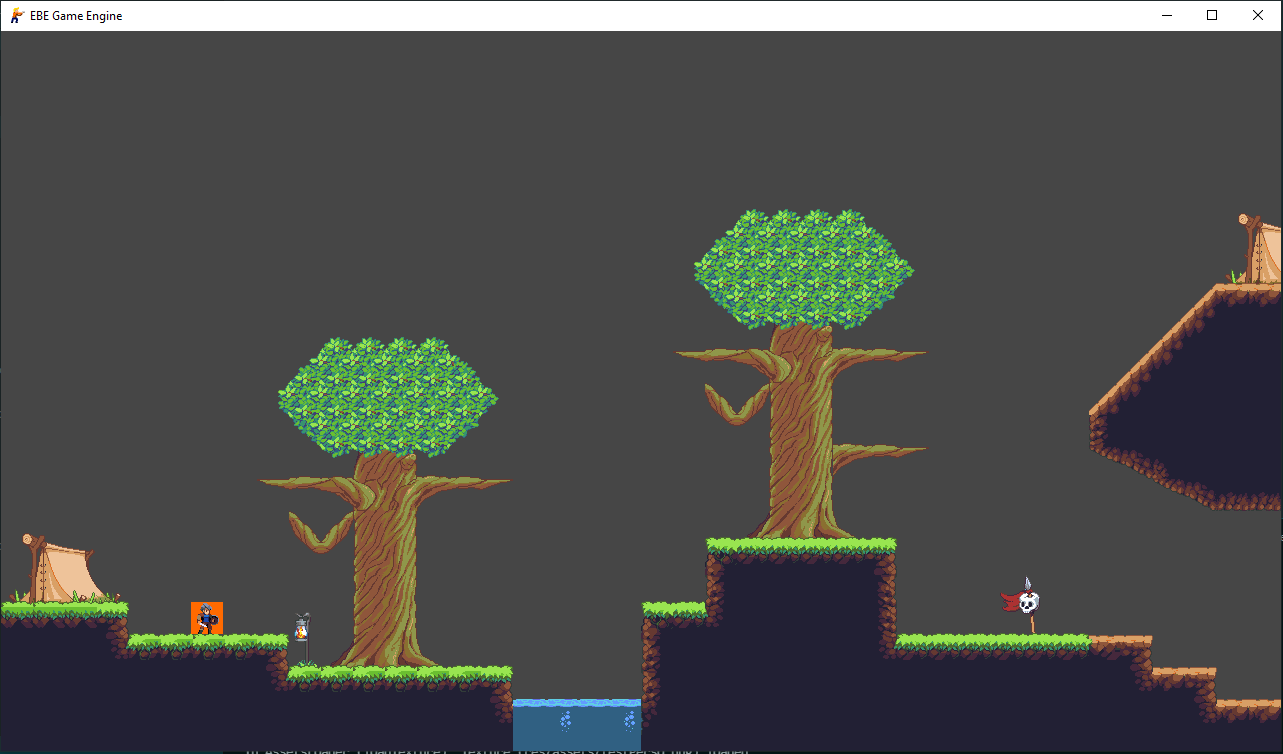
\includegraphics[scale=0.5]{etatJeuActuel.png}
\end{figure}
\\[0.5cm]
\indent Nous avons une carte, ainsi qu'un personnage pouvant se d\'eplacer librement sur cette derni\`ere.

\chapter{Analyse des besoins du projet}
Tout d'abord, j'ai entrepris des recherches sur les moteurs de jeu. Lors de ces derni\`eres, j'ai trouv\'e deux principaux mod\`eles de  moteur de jeu : \\
\begin{itemize}
\item Le mod\`ele bas\'e sur le paradigme de l'orient\'e objet;
\item Le mod\`ele bas\'e sur le paradigme de l'orient\'e donn\'ee, ;
\end{itemize}
\indent J'ai, dans un premier temps, pens\'e \`a choisir le paradigme orient\'e objet, \'etant donn\'e que nous l'avons beaucoup travaill\'e lors de ces derniers semestres. Mais apr\`es r\'eflexions, pour un moteur de jeu, l'orient\'e objet atteint ses limites. Prenons l'exemple simple suivant :
\\[0.2cm]
\begin{figure}[!h]
\centering
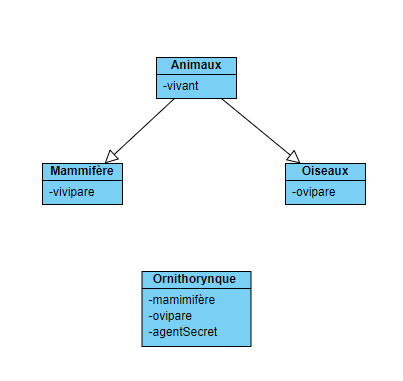
\includegraphics[scale=1]{illustrationOO.png}
\end{figure}
\newpage
\indent Dans cet exemple, nous avons une classe abstraite Animaux, dont h\'eritent deux classes, Mammif\`eres et Oiseaux. Les Mammif\`eres sont vivipares tandis que les Oiseaux sont ovipares. Dans ce cas, quid de l'Ornithorynque, ce mammif\`ere ovipare ? Il est vrai qu'en C++, il y a la possibilit\'e d'h\'eritages multiples, mais cela peut poser d'autres probl\`emes, comme dans l'exemple au dessus, si la classe Oiseaux a un attribut ailes, alors Ornithorynque ne devrait pas h\'eriter d'Oiseaux.
\\
\indent C'est l\`a o\`u le paradigme de l'orient\'e donn\'ee entre en jeu : \\[0.2cm]
\begin{figure}[!h]
\centering
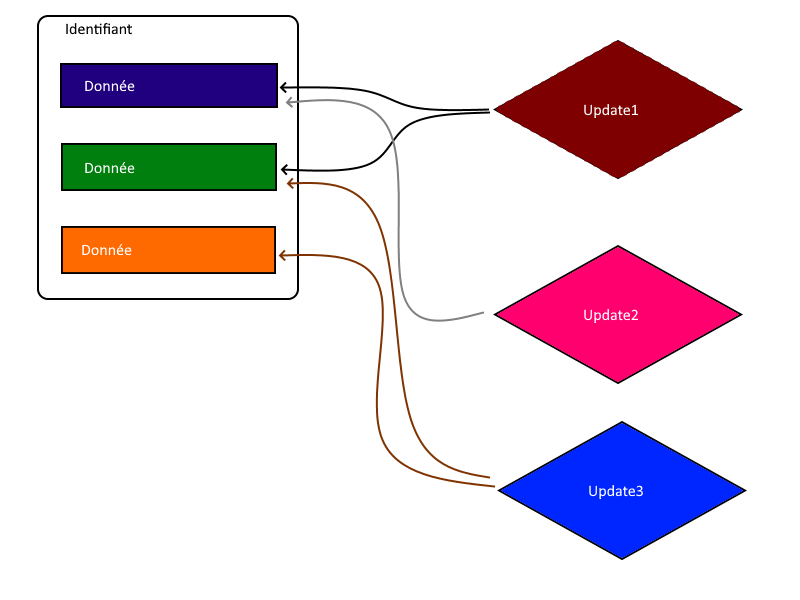
\includegraphics[scale=0.7]{illustrationOD.png}
\end{figure}
\\[0.5cm]
Dans ce paradigme, nous associons des donn\'ees \`a un identifiant, qui seront manipul\'e par des fonctions en les r\'ecup\'erant selon leur identifiant.
\\Dans le d\'eveloppement de jeux-vid\'eo, l'utilisation de ce paradigme m\`ene \`a un patterne nomm\'e ECS, pour Entity Component System. Les Entity (entit\'es) sont les identifiants, les Components (composants) sont les donn\'ees, et les Systems (syst\`emes) sont les fonctions.

\end{document}